% Simple poster (portrait)
% Author: Sofia Jijon (https://sjijon.github.io)
% Last Update: Sept 9, 2021
% Latest Version: https://github.com/sjijon/TeX-templates/tree/main/Tikzposter%20posters/Simple%20poster

\documentclass[a0paper,portrait,margin=0pt, colspace=24pt,subcolspace=0pt,blockverticalspace=36pt,innermargin=50pt]{tikzposter}
\usepackage[spanish,mexico]{babel}
\usepackage[latin9]{inputenc}
\usepackage[square,numbers]{natbib} 	% Bibliography manager
\usepackage{amsmath,amssymb}
\usepackage{lipsum}  				    % Random Text
\usepackage[colalign]{aligncolsatbottom}  %To align columns at bottom (!! please run 2 times)

%..............................................................................................................................................................................................
% Display
\tikzposterlatexaffectionproofoff 			
\usetikzlibrary{shapes.geometric,arrows.meta,positioning}  %Tikz Libraries

% Fonts
\usepackage{helvet}					% Sans-Serif
\renewcommand{\familydefault}{\sfdefault}	%

% Colors
	\definecolor{MyOrange}{rgb}{0, .14, 1.20}
	\definecolor{MyBrown}{rgb}{0, .14, 1.20}
	\definecolor{MyGreen}{rgb}{0.33, 0.42, 0.18}

% Theme
\usetheme{Default}
\definecolorstyle{MyStyle2016}{
	\definecolor{ColorOne}{named}{MyBrown} 
	\definecolor{ColorTwo}{named}{MyOrange}
	\definecolor{ColorThree}{named}{MyGreen}
}{
    % Title Colors
    \colorlet{titlebgcolor}{ColorOne}
    \colorlet{titlefgcolor}{white}
    % Background Colors
    \colorlet{backgroundcolor}{ColorOne!15}
    \colorlet{framecolor}{ColorOne}
    % Block Colors
    \colorlet{blocktitlebgcolor}{white}
    \colorlet{blocktitlefgcolor}{ColorTwo}
    \colorlet{blockbodybgcolor}{white}
    \colorlet{blockbodyfgcolor}{black}
    % Innerblock Colors
    \colorlet{innerblocktitlebgcolor}{ColorOne!15}
    \colorlet{innerblocktitlefgcolor}{black}
    \colorlet{innerblockbodybgcolor}{ColorOne!15}
    \colorlet{innerblockbodyfgcolor}{black}
    % Note colors
    \colorlet{notebgcolor}{ColorTwo!20}
    \colorlet{notefgcolor}{ColorTwo}
    \colorlet{notefrcolor}{ColorTwo}
 }

% Color style
\usecolorstyle{MyStyle2016}
%..............................................................................................................................................................................................
\title{An\'{a}lisis de contaminantes de San Nicol\'{a}s de los Garza}

\author{Pedro Alan Gonz\'{a}lez Ar\'{a}mbula - A01625308, Miguel \'{A}ngel Ch\'{a}vez Robles - A01620402, Francisco Leonid G\'{a}lvez Flores  - A01174385}

\institute{	Instituto Tecnol\'{o}gico y de Estudios Superiores de Monterrey. Monterrey, Nuevo Le\'{o}n}

%..............................................................................................................................................................................................
\begin{document}
%
%
%	HEAD
%
%....................................................................................
%
%	Title
%
\maketitle[width=0.96\linewidth,titletoblockverticalspace=36pt,linewidth=0,roundedcorners=10]

\begin{columns}

\column{0.5}

\block[titleleft,roundedcorners=16]{Introducci\'{o}n}{
	\raggedright
	El an\'{a}lisis de componentes principales es una t\'{e}cnica usada cuando se tienen datos con un alto n\'{u}mero de dimensiones y se desea encontrar un n\'{u}mero menor de variables no correlacionadas, denominadas ``componentes principales'' para representar la misma informaci\'{o}n. Estas son combinaciones lineales de las variables originales \textsuperscript{[2]}.  
}
%....................................................................................
%
%	Block
%
\block[titleleft,roundedcorners=16]{Base de datos}{
	\raggedright
	
	Se analizar\'{o}n los datos de contaminantes e indicadores meteoreol\'{o}gicos proporcionados por el  
     ``Sistema de Monitoreo Ambiental'' de la Direcci\'{o}n De Gesti\'{o}n Integral de la Calidad del Aire del Gobierno del Estado de Nuevo Le\'{o}n. La estaci\'{o}n analizada fue la estaci\'{o}n noreste, ubicada en San Nicol\'{a}s de los Garza, Nuevo Le\'{o}n. El periodo de tiempo usado para el an\'{a}lisis va del primero de agosto de 2018 al 31 de julio del 2019. Este periodo fue escogido debido a que en el an\'{a}lsis exploratorio este demostr\'{o} ser el m\'{a}s completo, pues ten\'{i}a el menor n\'{u}mero de datos faltantes.

}
%....................................................................................
%
%	Block
%
\block[titleleft,roundedcorners=16]{Metodolog\'{i}a\large\\An\'{a}lisis de valores propios}{
\raggedright

    Al realizar un an\'{a}lisis de componentes principales se busca encontrar $k$ variables que expliquen de buena manera las $p$ variables originales de manera que $k<p$. Este puede realizarse de 2 maneras: por matriz de correlaci\'{o}n y de covarianza; en nuestro caso se realiz\'{o} el an\'{a}lisis por matriz de correlaci\'{o}n pues las escalas de las variables no son iguales. Los valores propios, proporci\'{o}n de varianza explicada y varianza explicada acumulada por componente se muestran a continuaci\'{o}n.  

\centering

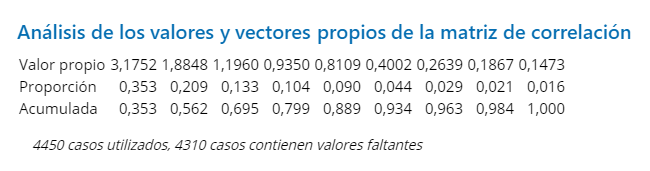
\includegraphics[scale=1.5]{Figures/analsisValoresVectores.png}

	\raggedright


Al momento de escoger cu\'{a}les $k$ componentes existen 2 t\'{e}cnicas bastante utilizadas, el ``Criterio de Kaiser-Guttman'', el cual sugiere escoger componentes principales cuyo valor propio $\lambda>1$ \textsuperscript{[1]}, alternativamente existe el criterio de varianza acumulada, el cual establece que deben tomarse $k$ componentes tales que la varianza acumulada de estos sea mayor o igual al 80\% de la varianza total. 
Esta se obtiene con la f\'{o}rmula mostrada a continuaci\'{o}n. 

\centering

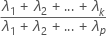
\includegraphics[scale=2.5]{Figures/acumulada.png} \textsuperscript{[3]}


\raggedright


En el an\'{a}lisis realizado se opt\'{o} por el criterio de la varianza acumulada, quedando con 5 componentes principales.
}

%..............................................................................................................................................................................................
%
%	CENTER COLUMN
%
\column{0.5}
%....................................................................................
%
% 	Block
%
\block[titleleft,roundedcorners=16]{\large Selecci\'{o}n de componentes principales}{
	\raggedright
	La gr\'{a}fica de sedimentaci\'{o}n representa la varianza acumulada de la matriz anterior.
	
	\centering
	
	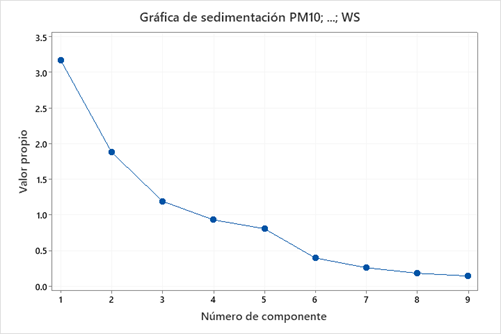
\includegraphics[scale=1.5]{Figures/sedimentacion.png}
	
			\raggedright

	Tras haber decidido usar 5 componentes principales, se obtiene la matriz de eigenvectores. Esta se interpreta como la carga que tiene cada variable sobre el componente. Esta carga puede ser tanto positiva como negativa. A su derecha se muestra la interpretaci\'{o}n gr\'{a}fica de las 2 primeras columnas 
	
	\centering
	
	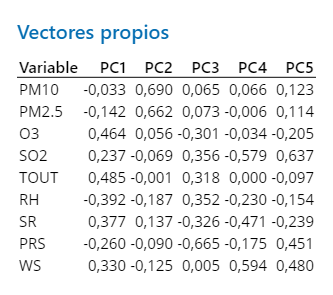
\includegraphics[scale=1.5]{Figures/vectoresPropios.png}
	
	\\
		\raggedright

	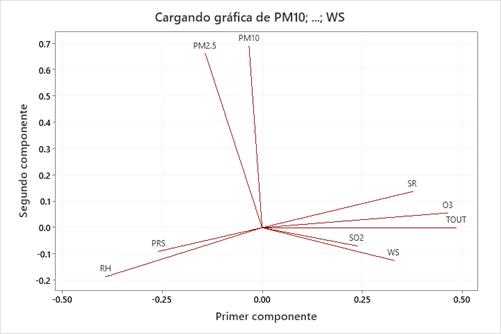
\includegraphics[scale=1.3]{Figures/cargas.png}
	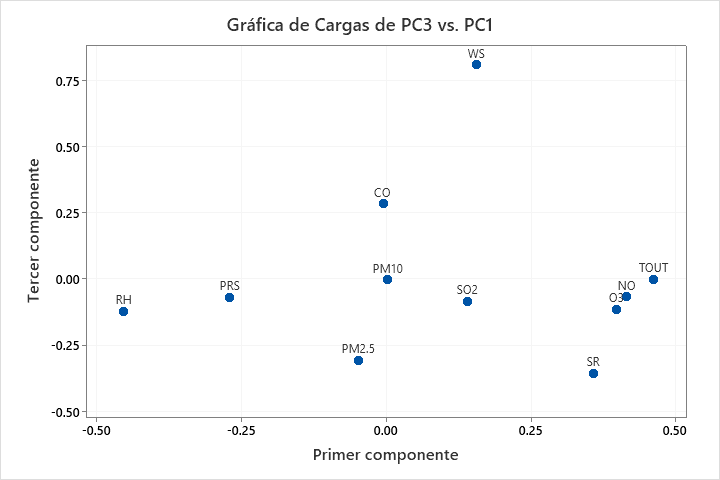
\includegraphics[scale=.69]{Figures/image.png}
	
	
 }
%....................................................................................
%
%	Block
%
\block[titleleft,roundedcorners=16]{\large Valores at\'{i}picos}{
	
	\raggedright
	
	Usando la distancia de Mahalanobis se determin\'{o} que los valores at\'{i}picos son todos los que se encuentren arriba de 4.116 de la misma. Existe un n\'{u}mero considerable de datos que cumplen este criterio.
	
	\centering
	
	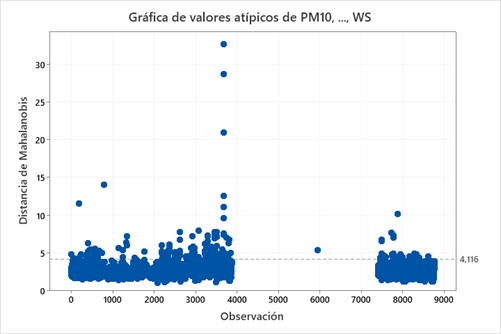
\includegraphics[scale=1.6]{Figures/atipicos.png}

}

%
\end{columns} 

\block[titleleft,roundedcorners=16]{Conclusiones}{

Se escogi\'{o} usar 5 componentes para describir de manera completa los datos originales, pues estos explican el 88.9\% de la varianza. No todos los componentes cumplen con el criterio de Kaiser-Guttman, lo cual puede esperarse de los datos, ya que estos tienen un comportamiento err\'{a}tico, son relativamente estacionales, adem\'{a}s existen grandes periodos sin lecturas y una cantidad considerable de valores at\'{i}picos. A futuro ser\'{i}a valioso realizar el mismo an\'{a}lisis utilizando variables transformadas. Adicionalmente se sugiere estudiar los valores at\'{i}picos encontrados para confirmar si estos se tratan de errores de captura, fen\'{o}menos naturales ocasionales, o si realmente el clima en San Nicol\'{a}s de los Garza tiene un comportamiento anormal. 
}
%..............................................................................................................................................................................................
%
%	FOOT
%
%....................................................................................
%
%	References
%
\block[titleleft,roundedcorners=16]{}{
\small
\begin{minipage}{0.7\linewidth}
	\nocite{*}

\bibliographystyle{abbrv}

\bibliography{biblio}

\end{minipage}
%....................................................................................
%
%	Logos
%
\begin{minipage}{0.3\linewidth}
\centering


\includegraphics[scale=0.4]{Figures/tecnologico-de-monterrey-blue.png}



\includegraphics[scale=0.4]{Figures/L-sima-CN-1.png}

\end{minipage}
}
%....................................................................................
%
%	My info
%



%}
\end{document}